%%%%%%%%%%%%%%%%%%%%%%%%%%%%%%%%%%%%%%%%%%%%%%%%%%%%%%%%%%%%%%%%%%%%%%%%%%%%%%%
%
% Tommy P. Keane
% Master of Science Thesis
% Department of Electrical and Microelectronic Engineering
% Rochester Institute of Technology
%
% April 2011
%
%
%
% Funded By: Lenel Systems Inc., A UTC Fire & Security Corporation
%
% Algorithm Intellectual Property Owned By: Lenel Systems Inc.
%
%
% http://www.tommypkeane.com
%
%%%%%%%%%%%%%%%%%%%%%%%%%%%%%%%%%%%%%%%%%%%%%%%%%%%%%%%%%%%%%%%%%%%%%%%%%%%%%%%

%%%%%%%%%%%%%%%%%%%%%%%%%%%%%%%%%%%%%%%%%%%%%%%%%%%%%%%%%%%%%%%%%%%%%%%%%%%%%%%
%
% CHAPTER 2
%
% SECTION 5: Camera Geometry
%
%%%%%%%%%%%%%%%%%%%%%%%%%%%%%%%%%%%%%%%%%%%%%%%%%%%%%%%%%%%%%%%%%%%%%%%%%%%%%%%


%%%%%%%%%%%%%%%%%%%%%%%%%%%%%%%%%%%%%%%%%%%%%%%%%%%%%%%%%%%%%%%%%%%%%%%%%%%%%%%
% BEGIN DOCUMENT

The previous Sections have presented the mathematics and concepts required for building the mutual information metric and applying it to digital images. The final major concept to understand in the theoretical development and motivation is how multiple views of a single scene can be related mathematically.

As the discussion has been already laid out, there are three distinct coordinate systems present in the mathematics discussed here. There are the scene coordinates, the camera (view) coordinates (the digital video), and the frame (image) coordinates. The camera view projects the real-world scene onto the 2-D spatial domain of the camera plane while preserving the time dimension (albeit sampled and quantized in all of these dimension), and the frame is an instance of the time dimension of the camera. Video compression concerns will be ignored in this development though they play a role in the success of the algorithm, but simplistically they can be thought of as  more quantization and interpolation. A diagram of the scene, views, and objects is presented in Figure \ref{sceneTerminology}.

\begin{figure}[h]
\centering
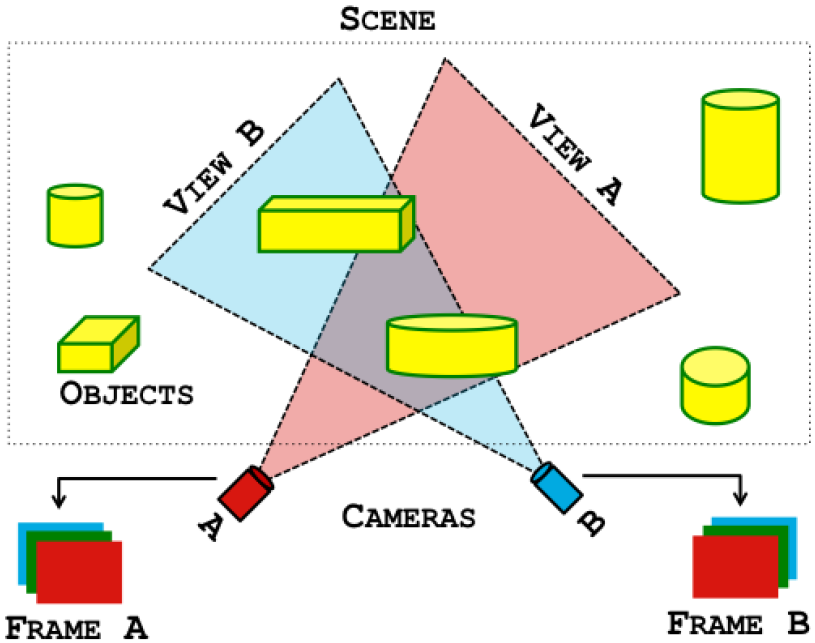
\includegraphics[width=.7\textwidth]{Terminology}
\caption{Terminology and structure of our application.}
\label{sceneTerminology}
\end{figure}

Understanding camera geometry is most easily understood by modeling the digital camera as a spatial projection system with a pinhole/point aperture \cite{Hartley2003}. Extending all of the following to realistic apertures would mostly just modify image spatial resolution and essentially creates a blurring effect on the results. Including this would only complicate the discussion as ray geometry would have to be abandoned for wavefront physics. So, again, the camera is thought of as a system that takes the light reflected and refracted off of the objects in the scene, allows it to pass through the point aperture (modeled as rays), and captures the light rays at the sample locations on the CCD array (which again has the Bayer filter in the case of color imagery). This model for a single camera is shown in Figure \ref{CameraModel}.

\begin{figure}[h]
\centering
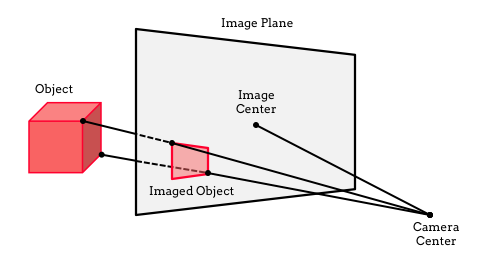
\includegraphics[width=.7\textwidth]{CameraModel}
\caption{Projective Camera System Model}
\label{CameraModel}
\end{figure}


There are the 3-D objects in the scene that become projected through the camera aperture (not shown for simplification) onto the camera's image plane as a 2-D imaged object. As the camera center moves in relation to the object in the scene, the projection of the object will change. Looking at Figure \ref{CameraModel}, our first constraint/assumption is that the cameras (the views) will remain stationary but these other cameras viewing the same scene will have distinct projections of the objects in the scene. In this diagram the object is highly symmetric so there will be many views that seem identical but real-world objects are not typically this symmetric; although they do have typically rigid shapes with relatively smooth textures, \ie{ }large areas of low entropy. Clearly for multiple views, the closer the camera centers are, the more similar the views will be. If the scene has many objects and a lot of 3-dimensional spatial variation, then it will require less and less distance between camera centers for the views to change significantly. Yet modeling a general scene as having a significant but not extensive amount of 3-dimensional variation can fall back to the discussion on regional PMFs, where the overlapping regions in the views will be similar enough in intensity or projected scene content that their PMFs should have a higher mutual information than any other combination of regions.


\begin{figure}[h]
\centering
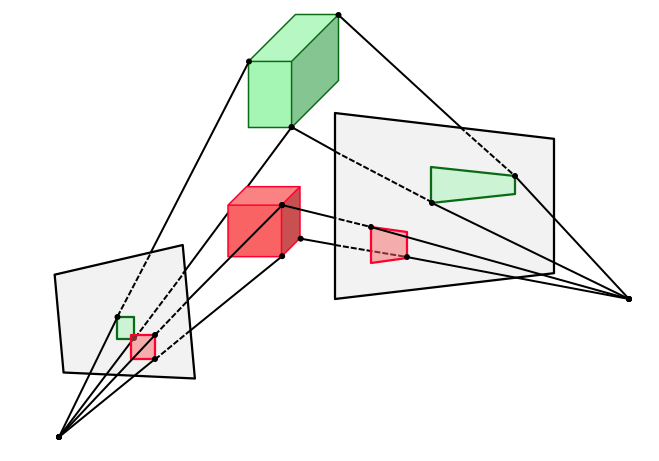
\includegraphics[width=.7\textwidth]{CameraOcclusion}
\caption{Multiple Projective Cameras Model}
\label{CameraOcclusion}
\end{figure}

In Figure \ref{CameraOcclusion} Camera A's image suffers from occlusion where the red block is covering a corner of the green block, as also indicated by the paths of the rays. There is also the effect of parallax, wherein with each view the distance between projected objects in the images varies based on the camera's distance to the objects in the scene. The red and green blocks appear very close together spatially in Camera A's view but are spaced far apart in Camera B's. Occlusion and parallax are not just characteristics of the views, they are characteristic of the entire scenario: the scene, its objects, and the views.

So ultimately what is applicable to this algorithm that needs to be understood about camera geometry? Projection is the main thrust of this discussion, even though multi-view geometry is an extremely rich and interesting topic, because the goal of this algorithm is to generate convincing panoramas of realistic scenes, automatically. Views like those modeled in Figure \ref{CameraOcclusion} are certainly relatable through epipolar constraints and use of a Fundamental matrix \cite{Hartley2003}, but they would not produce a 2-D panorama. Clearly there must be some initial restriction, in the basic theory, where camera centers are not at angles of rotation much beyond 45\textsuperscript{o} to one another with respect to their views. Realistically, \ie{ }in practice, this is a general and typical scenario as cameras will be placed along typically rectangular structures such as buildings and fence lines or in hallways. Yet even in these scenarios, there will be significant occurrences of occlusion, and differences in occlusion between views stemming from parallax discrepancies. With significant occlusion disparity, any point-to-point correspondence algorithm that considered occluded and non-occluded features would have added ambiguity in attempting correspondence in an already unknown scene. The more complex the scene is, such as irregular shaped objects and large variations in 3-dimensional arrangements, there will be many points existing in one view that do not exist in the other but could seem to, mathematically. This is the foundational motivation for designing the WFMI algorithm as a region-based correspondence rather than a point-based correspondence algorithm. Point-to-point correspondence can certainly allow for more realistic deformations, but it can also allow for extremely unrealistic deformations. Given that that corner of the green box was found in one view and not the other, it could be searched for in the second view and accidentally corresponded to some other box's corner in the scene. Using that relationship to develop the homography or transformation between the views \cite{Hartley2003} can produce extreme inaccuracy.

It is important to understand that occlusion and parallax are extremely difficult to model, but occur extremely often in realistic scenarios. With no known relationship between camera locations, the WFMI algorithm took this knowledge of multi-view geometry and its constraints to assume that even though there will not be a full set of points in an overlap region that can be corresponded, the structure and arrangement of objects will be there, and that's what should be searched for. This is why it is a region based algorithm, as it compares scenes based on the structure and arrangement of the objects, not the exact location of all the points on the objects. That is also why it is so successful despite only searching for an affine relationship between views more accurately relatable by a projective homography or a Fundamental matrix.

%%%%%%%%%%%%%%%%%%%%%%%%%%%%%%%%%%%%%%%%%%%%%%%%%%%%%%%%%%%%%%%%%%%%%%%%%%%%%%%
% END OF DOCUMENT

